\documentclass[a4paper,12pt]{article}
\usepackage{graphicx}
\usepackage{amsmath}
\usepackage[margin=1in]{geometry}
\usepackage{amsmath, amssymb}
\usepackage{float}
\usepackage{caption}
\usepackage{subcaption}
\usepackage{xcolor}
\usepackage{fancyhdr}
\usepackage{array}
\usepackage{float}
\definecolor{darkskyblue}{rgb}{0.0, 0.5, 1.0}
\definecolor{skyblue}{RGB}{135, 206, 235}

\geometry{a4paper, top=0.7in, left=1in, right=1in, bottom=1in}

\begin{document}

\pagestyle{empty} % Start with empty page style

\thispagestyle{fancy} % Apply fancy style only to the first page
\fancyhf{} % Clear header and footer
\renewcommand{\headrulewidth}{0pt} % Remove header rule
\fancyhead[L]{% Left header
        
\includegraphics[width=8cm, height=1.7cm]{img3.png} 
        }
\fancyhead[R]{% Right header
    Name: A.Likhitha \\
    Batch: COMETFWC019\\
    Date: 17 may 2025
}

\vspace{1cm}
\begin{center}

    {\LARGE \textbf{\textcolor{darkskyblue}{\\  GATE QUESTION \\ ECE 2010 Q52}}}
\end{center}
\noindent\textbf{Statement for Linked Answer Questions: 52 } \\[0.3cm]
The following Karnaugh map represents a function \( F \).\\[0.3cm]
\begin{center}
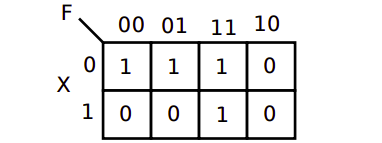
\includegraphics[width=0.4\textwidth]{l.png} \\[0.4cm]
\end{center}
\noindent\textbf{52.} A minimized form of the function \( F \) is\\[0.3cm]
\hspace*{1cm}(A)\quad \( F = \overline{X}Y + YZ \)
\hspace*{1cm}(B)\quad \( F = \overline{X}\,\overline{Y} + YZ \)\\
\hspace*{1cm}(C)\quad \( F = \overline{\overline{X}}\,\overline{Y} + Y\overline{Z} \)
\hspace*{1cm}(D)\quad \( F = \overline{X}Y + \overline{Y}Z \)\\[0.3cm]
\noindent\textbf{Answer:} (B)\\[1cm]
\textbf{Solution:}
\begin{center}
   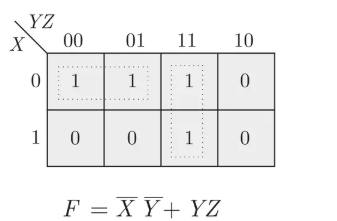
\includegraphics[width=0.4\textwidth]{q.png} 
\end{center}
\textbf{Group 1 – Horizontal Pair (X = 0):}
\begin{itemize}
    \item Covers cells: $(X=0, Y=0, Z=0)$ and $(X=0, Y=0, Z=1)$
    \item Minterms: $X'Y'Z'$, $X'Y'Z$
    \item Common literals: $X'=1$, $Y'=1$, $Z$ varies
    \item \textbf{Simplified term:} $X'Y'$
\end{itemize}
\hspace{-0.5em}
\textbf{Group 2 – Vertical Pair (YZ = 11):}
\begin{itemize}
    \item Covers cells: $(X=0, Y=1, Z=1)$ and $(X=1, Y=1, Z=1)$
    \item Minterms: $X'YZ$, $XYZ$
    \item Common literals: $Y=1$, $Z=1$, $X$ varies
    \item \textbf{Simplified term:} $YZ$
\end{itemize}

\bigskip

\textbf{Final Simplified SOP Expression:}
\[
F = X'Y' + YZ
\]

\textbf{Answer: (B)}
\end{document}
\end{document}
